%% This style is provided for the ICSE 2015 main conference,
%% ICSE 2015 co-located events, and ICSE 2015 workshops.

%% bare_conf_ICSE15.tex
%% V1.4
%% 2014/05/22


%% This is a skeleton file demonstrating the use of IEEEtran.cls
%% (requires IEEEtran.cls version 1.7 or later) with an IEEE conference paper.
%%
%% Support sites:
%% http://www.michaelshell.org/tex/ieeetran/
%% http://www.ctan.org/tex-archive/macros/latex/contrib/IEEEtran/
%% and
%% http://www.ieee.org/

%%*************************************************************************
%% Legal Notice:
%% This code is offered as-is without any warranty either expressed or
%% implied; without even the implied warranty of MERCHANTABILITY or
%% FITNESS FOR A PARTICULAR PURPOSE!
%% User assumes all risk.
%% In no event shall IEEE or any contributor to this code be liable for
%% any damages or losses, including, but not limited to, incidental,
%% consequential, or any other damages, resulting from the use or misuse
%% of any information contained here.
%%
%% All comments are the opinions of their respective authors and are not
%% necessarily endorsed by the IEEE.
%%
%% This work is distributed under the LaTeX Project Public License (LPPL)
%% ( http://www.latex-project.org/ ) version 1.3, and may be freely used,
%% distributed and modified. A copy of the LPPL, version 1.3, is included
%% in the base LaTeX documentation of all distributions of LaTeX released
%% 2003/12/01 or later.
%% Retain all contribution notices and credits.
%% ** Modified files should be clearly indicated as such, including  **
%% ** renaming them and changing author support contact information. **
%%
%% File list of work: IEEEtran.cls, IEEEtran_HOWTO.pdf, bare_adv.tex,
%%                    bare_conf.tex, bare_jrnl.tex, bare_jrnl_compsoc.tex
%%*************************************************************************

% *** Authors should verify (and, if needed, correct) their LaTeX system  ***
% *** with the testflow diagnostic prior to trusting their LaTeX platform ***
% *** with production work. IEEE's font choices can trigger bugs that do  ***
% *** not appear when using other class files.                            ***
% The testflow support page is at:
% http://www.michaelshell.org/tex/testflow/



% Note that the a4paper option is mainly intended so that authors in
% countries using A4 can easily print to A4 and see how their papers will
% look in print - the typesetting of the document will not typically be
% affected with changes in paper size (but the bottom and side margins will).
% Use the testflow package mentioned above to verify correct handling of
% both paper sizes by the user's LaTeX system.
%
% Also note that the "draftcls" or "draftclsnofoot", not "draft", option
% should be used if it is desired that the figures are to be displayed in
% draft mode.
%
\documentclass[conference]{IEEEtran}
%
% If IEEEtran.cls has not been installed into the LaTeX system files,
% manually specify the path to it like:
% \documentclass[conference]{../sty/IEEEtran}





% Some very useful LaTeX packages include:
% (uncomment the ones you want to load)


% *** MISC UTILITY PACKAGES ***
%
%\usepackage{ifpdf}
% Heiko Oberdiek's ifpdf.sty is very useful if you need conditional
% compilation based on whether the output is pdf or dvi.
% usage:
% \ifpdf
%   % pdf code
% \else
%   % dvi code
% \fi
% The latest version of ifpdf.sty can be obtained from:
% http://www.ctan.org/tex-archive/macros/latex/contrib/oberdiek/
% Also, note that IEEEtran.cls V1.7 and later provides a builtin
% \ifCLASSINFOpdf conditional that works the same way.
% When switching from latex to pdflatex and vice-versa, the compiler may
% have to be run twice to clear warning/error messages.






% *** CITATION PACKAGES ***
%
%\usepackage{cite}
% cite.sty was written by Donald Arseneau
% V1.6 and later of IEEEtran pre-defines the format of the cite.sty package
% \cite{} output to follow that of IEEE. Loading the cite package will
% result in citation numbers being automatically sorted and properly
% "compressed/ranged". e.g., [1], [9], [2], [7], [5], [6] without using
% cite.sty will become [1], [2], [5]--[7], [9] using cite.sty. cite.sty's
% \cite will automatically add leading space, if needed. Use cite.sty's
% noadjust option (cite.sty V3.8 and later) if you want to turn this off.
% cite.sty is already installed on most LaTeX systems. Be sure and use
% version 4.0 (2003-05-27) and later if using hyperref.sty. cite.sty does
% not currently provide for hyperlinked citations.
% The latest version can be obtained at:
% http://www.ctan.org/tex-archive/macros/latex/contrib/cite/
% The documentation is contained in the cite.sty file itself.






% *** GRAPHICS RELATED PACKAGES ***
%
\ifCLASSINFOpdf
   \usepackage[pdftex]{graphicx}
  % declare the path(s) where your graphic files are
  % \graphicspath{{../pdf/}{../jpeg/}}
  % and their extensions so you won't have to specify these with
  % every instance of \includegraphics
  % \DeclareGraphicsExtensions{.pdf,.jpeg,.png}
\else
  % or other class option (dvipsone, dvipdf, if not using dvips). graphicx
  % will default to the driver specified in the system graphics.cfg if no
  % driver is specified.
  % \usepackage[dvips]{graphicx}
  % declare the path(s) where your graphic files are
  % \graphicspath{{../eps/}}
  % and their extensions so you won't have to specify these with
  % every instance of \includegraphics
  % \DeclareGraphicsExtensions{.eps}
\fi
% graphicx was written by David Carlisle and Sebastian Rahtz. It is
% required if you want graphics, photos, etc. graphicx.sty is already
% installed on most LaTeX systems. The latest version and documentation can
% be obtained at:
% http://www.ctan.org/tex-archive/macros/latex/required/graphics/
% Another good source of documentation is "Using Imported Graphics in
% LaTeX2e" by Keith Reckdahl which can be found as epslatex.ps or
% epslatex.pdf at: http://www.ctan.org/tex-archive/info/
%
% latex, and pdflatex in dvi mode, support graphics in encapsulated
% postscript (.eps) format. pdflatex in pdf mode supports graphics
% in .pdf, .jpeg, .png and .mps (metapost) formats. Users should ensure
% that all non-photo figures use a vector format (.eps, .pdf, .mps) and
% not a bitmapped formats (.jpeg, .png). IEEE frowns on bitmapped formats
% which can result in "jaggedy"/blurry rendering of lines and letters as
% well as large increases in file sizes.
%
% You can find documentation about the pdfTeX application at:
% http://www.tug.org/applications/pdftex


\makeatletter
\newenvironment{tablehere}
  {\def\@captype{table}}
  {}

\newenvironment{figurehere}
  {\def\@captype{figure}}
  {}
\makeatother


% *** MATH PACKAGES ***
%
%\usepackage[cmex10]{amsmath}
% A popular package from the American Mathematical Society that provides
% many useful and powerful commands for dealing with mathematics. If using
% it, be sure to load this package with the cmex10 option to ensure that
% only type 1 fonts will utilized at all point sizes. Without this option,
% it is possible that some math symbols, particularly those within
% footnotes, will be rendered in bitmap form which will result in a
% document that can not be IEEE Xplore compliant!
%
% Also, note that the amsmath package sets \interdisplaylinepenalty to 10000
% thus preventing page breaks from occurring within multiline equations. Use:
%\interdisplaylinepenalty=2500
% after loading amsmath to restore such page breaks as IEEEtran.cls normally
% does. amsmath.sty is already installed on most LaTeX systems. The latest
% version and documentation can be obtained at:
% http://www.ctan.org/tex-archive/macros/latex/required/amslatex/math/





% *** SPECIALIZED LIST PACKAGES ***
%
%\usepackage{algorithmic}
% algorithmic.sty was written by Peter Williams and Rogerio Brito.
% This package provides an algorithmic environment fo describing algorithms.
% You can use the algorithmic environment in-text or within a figure
% environment to provide for a floating algorithm. Do NOT use the algorithm
% floating environment provided by algorithm.sty (by the same authors) or
% algorithm2e.sty (by Christophe Fiorio) as IEEE does not use dedicated
% algorithm float types and packages that provide these will not provide
% correct IEEE style captions. The latest version and documentation of
% algorithmic.sty can be obtained at:
% http://www.ctan.org/tex-archive/macros/latex/contrib/algorithms/
% There is also a support site at:
% http://algorithms.berlios.de/index.html
% Also of interest may be the (relatively newer and more customizable)
% algorithmicx.sty package by Szasz Janos:
% http://www.ctan.org/tex-archive/macros/latex/contrib/algorithmicx/




% *** ALIGNMENT PACKAGES ***
%
%\usepackage{array}
% Frank Mittelbach's and David Carlisle's array.sty patches and improves
% the standard LaTeX2e array and tabular environments to provide better
% appearance and additional user controls. As the default LaTeX2e table
% generation code is lacking to the point of almost being broken with
% respect to the quality of the end results, all users are strongly
% advised to use an enhanced (at the very least that provided by array.sty)
% set of table tools. array.sty is already installed on most systems. The
% latest version and documentation can be obtained at:
% http://www.ctan.org/tex-archive/macros/latex/required/tools/


%\usepackage{mdwmath}
%\usepackage{mdwtab}
% Also highly recommended is Mark Wooding's extremely powerful MDW tools,
% especially mdwmath.sty and mdwtab.sty which are used to format equations
% and tables, respectively. The MDWtools set is already installed on most
% LaTeX systems. The lastest version and documentation is available at:
% http://www.ctan.org/tex-archive/macros/latex/contrib/mdwtools/


% IEEEtran contains the IEEEeqnarray family of commands that can be used to
% generate multiline equations as well as matrices, tables, etc., of high
% quality.


%\usepackage{eqparbox}
% Also of notable interest is Scott Pakin's eqparbox package for creating
% (automatically sized) equal width boxes - aka "natural width parboxes".
% Available at:
% http://www.ctan.org/tex-archive/macros/latex/contrib/eqparbox/





% *** SUBFIGURE PACKAGES ***
%\usepackage[tight,footnotesize]{subfigure}
% subfigure.sty was written by Steven Douglas Cochran. This package makes it
% easy to put subfigures in your figures. e.g., "Figure 1a and 1b". For IEEE
% work, it is a good idea to load it with the tight package option to reduce
% the amount of white space around the subfigures. subfigure.sty is already
% installed on most LaTeX systems. The latest version and documentation can
% be obtained at:
% http://www.ctan.org/tex-archive/obsolete/macros/latex/contrib/subfigure/
% subfigure.sty has been superceeded by subfig.sty.



%\usepackage[caption=false]{caption}
%\usepackage[font=footnotesize]{subfig}
% subfig.sty, also written by Steven Douglas Cochran, is the modern
% replacement for subfigure.sty. However, subfig.sty requires and
% automatically loads Axel Sommerfeldt's caption.sty which will override
% IEEEtran.cls handling of captions and this will result in nonIEEE style
% figure/table captions. To prevent this problem, be sure and preload
% caption.sty with its "caption=false" package option. This is will preserve
% IEEEtran.cls handing of captions. Version 1.3 (2005/06/28) and later
% (recommended due to many improvements over 1.2) of subfig.sty supports
% the caption=false option directly:
%\usepackage[caption=false,font=footnotesize]{subfig}
%
% The latest version and documentation can be obtained at:
% http://www.ctan.org/tex-archive/macros/latex/contrib/subfig/
% The latest version and documentation of caption.sty can be obtained at:
% http://www.ctan.org/tex-archive/macros/latex/contrib/caption/




% *** FLOAT PACKAGES ***
%
%\usepackage{fixltx2e}
% fixltx2e, the successor to the earlier fix2col.sty, was written by
% Frank Mittelbach and David Carlisle. This package corrects a few problems
% in the LaTeX2e kernel, the most notable of which is that in current
% LaTeX2e releases, the ordering of single and double column floats is not
% guaranteed to be preserved. Thus, an unpatched LaTeX2e can allow a
% single column figure to be placed prior to an earlier double column
% figure. The latest version and documentation can be found at:
% http://www.ctan.org/tex-archive/macros/latex/base/



%\usepackage{stfloats}
% stfloats.sty was written by Sigitas Tolusis. This package gives LaTeX2e
% the ability to do double column floats at the bottom of the page as well
% as the top. (e.g., "\begin{figure*}[!b]" is not normally possible in
% LaTeX2e). It also provides a command:
%\fnbelowfloat
% to enable the placement of footnotes below bottom floats (the standard
% LaTeX2e kernel puts them above bottom floats). This is an invasive package
% which rewrites many portions of the LaTeX2e float routines. It may not work
% with other packages that modify the LaTeX2e float routines. The latest
% version and documentation can be obtained at:
% http://www.ctan.org/tex-archive/macros/latex/contrib/sttools/
% Documentation is contained in the stfloats.sty comments as well as in the
% presfull.pdf file. Do not use the stfloats baselinefloat ability as IEEE
% does not allow \baselineskip to stretch. Authors submitting work to the
% IEEE should note that IEEE rarely uses double column equations and
% that authors should try to avoid such use. Do not be tempted to use the
% cuted.sty or midfloat.sty packages (also by Sigitas Tolusis) as IEEE does
% not format its papers in such ways.





% *** PDF, URL AND HYPERLINK PACKAGES ***
%
%\usepackage{url}
% url.sty was written by Donald Arseneau. It provides better support for
% handling and breaking URLs. url.sty is already installed on most LaTeX
% systems. The latest version can be obtained at:
% http://www.ctan.org/tex-archive/macros/latex/contrib/misc/
% Read the url.sty source comments for usage information. Basically,
% \url{my_url_here}.





% *** Do not adjust lengths that control margins, column widths, etc. ***
% *** Do not use packages that alter fonts (such as pslatex).         ***
% There should be no need to do such things with IEEEtran.cls V1.6 and later.
% (Unless specifically asked to do so by the journal or conference you plan
% to submit to, of course. )


% correct bad hyphenation here
\hyphenation{op-tical net-works semi-conduc-tor}


\begin{document}

\title{A Token Frequency Based Code Clone Detection}

\author{\IEEEauthorblockN{He Feng\IEEEauthorrefmark{1},
Liuqing Li\IEEEauthorrefmark{2},
}
\IEEEauthorblockA{\IEEEauthorrefmark{1}Department of Physics,\\
Virginia Tech,
Blacksburg, VA, 24061\\ Email: fenghe@vt.edu}
\IEEEauthorblockA{\IEEEauthorrefmark{2}Department of Computer Science,\\
Virginia Tech,
Blacksburg, VA, 24061\\ Email: liuqing@vt.edu}
}

\maketitle


\begin{abstract}
%\boldmath
Code clone detection remains an active topic in software enginnering. It is not only common in the programming process, but also leading to low maintainability. 
In this paper, we propose a simple and efficient tool in Java to detect cloned codes, basing on the token frequency in source code. Our tool extracts variables in each block, performs pretreatment on them, as well as counts keywords and symbols. After transforming these pieces of information into lists, different weights are given to these components, then a similarity algorithm is introduced to find out similar codes. 
As a counting-based detection tool, it compares lists of names and numbers instead of source code directly, so we can expect less time cost compared to other detection tools. Also components have different weights, thus precision and recall can be maintained to some extent.
\end{abstract}

\section{Introduction}

It is very common that people clone codes in their programs, i.e. reuse some code fragments by copying with or without modification in the coding process. 
Previous research shows a significant fraction of the code being cloned even in some well-known software systems. The fraction of duplicated code in X Windows System is about 19\%\cite{cloneinsys1}, while in some core parts of Linux the number is between 15\% and 25\%\cite{cloneinsys2}. 
Even if code clone can improve the efficiency of a program in some ways, for example, reducing execution time for no need to call functions, it is quite difficult for developers to maintain a software in its life cycle: if fixing a bug, adding or cutting a feature, it has to be applied to all the similar parts. To solve this problem, clone detection has become an important tool for programmers, since it is much easier if provided all the copied parts when making a change.

A number of techniques and tools have been implemented, using various algorithms to find out code clones in different level. Token-based method shows a good comprehensive performance among all of them. However, every tool has its own limitations, just like the time cost of CCFinder. Then we provoked our research, to develop and implement a scalable clone detection based on tokens to detect code clone in token variation and statement modification.

While many researchers have done similar job before, our tool is new: since most developers would not make dramatic changes in code clone process except for some tokens such as keywords, types, variables and operators, we try to design and improve a simple statistical method to calculate the similarity between code fragments. Specifically, to detect whether fragment A is a clone of fragment B or not, we transform the two 


first we tokenize each fragment, design a flexible token filter, and compare the frequencies of them.




The more detailed idea is like below:
first the source code will be divided into fragments, for each fragment, any useful tokens, such as types, variables, identifiers, operators, will be counted, so the information is transformed into a list of names and numbers. 
Next is pretreatment of variable names, take fragments A and B, compare and find out similar variables using n-gram, here we assume that in actual cases, which usually contain a large amount of codes, variable names have to make sense, which means, no a's and b's, but something like StudentName and ClassAverage.
After finding matching variable names, we can compare the list, by putting different weights on different tokens, the accuracy is enhanced, and this similarity algorithm can be improved after actual testing.
Finall is setting up the threshold, which can also be decided after actual testing.

Our tool has its own advantages: the first part of this process is just counting, which has very low time cost; the next part is to find out similar variable names, which is the most time-consuming part in our process, but is still not complicated; the last part is to compare lists of names and numbers, which is simple math and pretty straightforward. For the whole process, we can expect low time cost.

For a counting based detection tool with low time cost, the accuracy can still be maintained to some extent, in our algorithm, the weighting part does contribute.

Our solution is new and we believe it's aggressive in clone detection field.


\section{Background}

To detect cloned codes, the first thing is to know clone types: there are two main kinds of similarity between code fragments. The first kind has textual similarity, and often comes from copying and pasting. Textual similarity can fall into three types: 
\begin{itemize}
\item Type 1 simply includes the variations in whitespace, layout and comments. 
\item Type 2 allows more variations in identifiers, literals and types, in addition to Type 1.
\item Type 3 contains Type 2 and allows further modifications such as changed, added or removed statements. 
\end{itemize}

An example of Type 1, 2, 3 clones is shown in Fig \ref{fig:TOC}. 

The second main kind is functional similarity. Functional similarity is described by Type 4 clone, or semantic clone, which is more complicated. 
\begin{itemize}
\item In Type 4 code fragments perform the same computation but are implemented in different ways. 
\end{itemize}

Few tools have been developed to detect Type 4 clones so far.\\


\begin{figurehere}
\centering 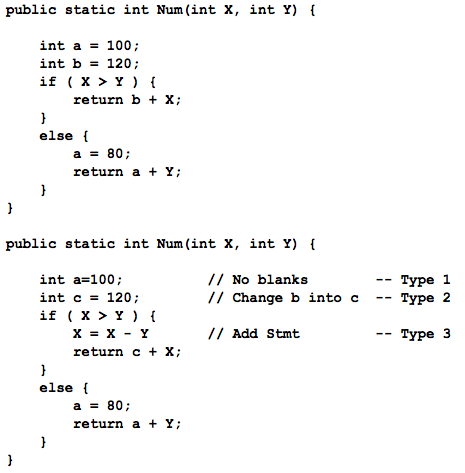
\includegraphics[width=0.4\textwidth]{graph2_1} \caption{Types of Clone} \label{fig:TOC}
\end{figurehere}

Based on the cloned types, researchers have developed different techniques and tools. 
\begin{itemize}
\item Text based, which means comparing whole lines to each other textually. 
\item Token based, it is still line-based comparision, but each sequence is summarized by a functor that abstracts the identifiers and literals, this encoding process preserves the structure of the whole sentence.
\item Metric based, by gathering different metrics for code fragments, these metric vectors are compared.
\item Tree based, usually means the abstract syntax trees(AST), a program is transformed into an abstract syntax tree, then the leaves and subtrees are compared.
\item Graph based, for example, program dependency graphs(PDG), control and data flow dependencies of a function can be represented by a program dependency graph, and comparision of subgraphs will be performed.
\end{itemize}

There are also other techniques but will not be discussed here.
Among all the techniques and tools, token-based method performs well in both clone type detection and time cost.


\section{Related Work}

Many token-based methods have been developed, like CCFinder\cite{CCFinder}, CMCD\cite{CMCD},  Boreas\cite{Boreas}, RTF\cite{RTF}. 

CCFinder is a classical tool, it first makes a parameter-replacement, like replaces identifiers with a token, and compares each code portion to all other portions. This is very long and detailed comparision, which results in a high accuracy, however that could also costs a huge amount of time.

CMCD uses Count Matrix, it counts many aspects for each variable, and constructs a count vector for that variable, then the count vectors are compared to find out corresponding variables. This method works well in extracting variables those are copied but in different names, but is doesn't include other contributions, like keywords and symbols.

Boreas is based on CMCD, it uses CMCD to compare variables, as well as taking keywords and symbols into account, but still has room for improvement, both in executing time, and detection accuracy. 

RTF uses flexible tokenization, but it doesn't use acess modifiers like \textbf{private, protected, public} and type names \textbf{int, short, long, float, double}, so it loses a lot of imformation.


%\section{Conclusion}
%The conclusion goes here.


% conference papers do not normally have an appendix

% use section* for acknowledgement
%\section*{Acknowledgment}
%
%
%The authors would like to thank...

% references section

\begin{thebibliography}{10}

\bibitem{cloneinsys1}
Brenda S. Baker, \emph{On Finding Duplication and Near-Duplication in Large Software Systems}

\bibitem{cloneinsys2}
G. Antoniola, U. Villanob, E. Merloc, M. Di Penta, \emph{Analyzing cloning evolution in the Linux kernel}

\bibitem{CCFinder}
T. Kamiya, S. Kusumoto and K. Inoue, \emph{A Token-based Code Clone Detection Tool - CCFinder and Its Empirical Evaluation}

\bibitem{CMCD}
Y. Yuan and Y. Guo, \emph{CMCD: Count Matrix based Code Clone Detection}

\bibitem{Boreas}
Y. Yuan and Y. Guo, \emph{Boreas: An Accurate and Scalable Token-Based Approach to Code Clone Detection}

\bibitem{RTF}
H. A. Basit, S. J. Puglisi, W. F. Smyth, A. Turpin and S. Jarzabel, \emph{Efficient Token Based Clone Detection with Flexible Tokenization}

\end{thebibliography}

\end{document}


